\documentclass[UTF8]{ctexart}
\usepackage{geometry}
\usepackage{listings}
\usepackage{xcolor}
\usepackage{graphicx}
\usepackage{float}
\usepackage{multirow}
\usepackage{array}
\usepackage{longtable}
\usepackage{hyperref}
\usepackage{ctex}

\geometry{a4paper,scale=0.8}
\lstset{
    numbers=left, %设置行号位置
    numberstyle=\tiny, %设置行号大小
    keywordstyle=\color{blue}, %设置关键字颜色
    commentstyle=\color[cmyk]{1,0,1,0}, %设置注释颜色
    frame=single, %设置边框格式
    escapeinside=``, %逃逸字符(1左面的键),用于显示中文
    breaklines, %自动折行
    extendedchars=false, %解决代码跨页时,章节标题,页眉等汉字不显示的问题
    xleftmargin=2em,xrightmargin=2em, aboveskip=1em, %设置边距
    tabsize=4, %设置tab空格数
    showspaces=false %不显示空格
    }
\hypersetup{
    colorlinks=true,
    linkcolor=black,
    citecolor=black
}
\title{计算机系统结构实验报告\\实验6}

\date{\today}


\begin{document}
\maketitle
\thispagestyle{empty}
\begin{abstract}
    本实验以实验3、4实现的功能模块以及实验5实现的类MIPS单周期处理器为基础,对部分功能模块进行了修改,增添高速缓存模块,并将支持的指令扩展到31条。此外,为实现流水线处理器,本实验增加了段寄存器,使用前向通路(forwarding)与流水线停顿(stall)来解决流水线冒险,通过预测不转移(predict-not-taken)策略提高流水线性能。最后,本实验将通过软件仿真的形式让处理器运行指令,以此进行实验结果的验证。
\end{abstract}  
\tableofcontents
\clearpage

\section{实验目的}
\begin{enumerate}
    \item 理解 CPU Pipeline,了解流水线冒险(hazard)及相关性,设计基础流水线CPU
    \item 设计支持停顿的流水线 CPU,通过检测竞争并插入停顿(Stall)机制解决数据冒险、控制竞争和结构冒险
    \item 增加前向传递机制解决数据竞争,减少因数据竞争带来的流水线停顿延时
    \item 通过predict-not-taken或延时转移策略解决控制冒险/竞争,减少控制竞争带来的流水线停顿延时
    \item 将CPU支持的指令数量从16条扩充为31条,使处理器功能更加丰富
    \item 设计并实现高速缓存
    \item 功能仿真
\end{enumerate}
\section{原理分析}
\subsection{功能模块原理分析}
\subsubsection{主控制器模块}\label{sec:design-ctr}
主控制器(Ctr)的输入为指令的操作码(opCode)字段,主控制器模块对操作码进行译码,向ALU控制器、寄存器、数据选择器等部件输出正确的控制信号。\par
本实验中,主控制器模块可以识别R型指令和MIPS指令集中其他所有指令并输出对应的控制信号。相比于实验5中的主控制器模块,为了提高流水线执行JR指令的性能,需要在指令译码(ID)阶段完成JR指令的识别,而实验5中jrSign信号由ALUCtr产生,无法在ID阶段完成,所以在本实验中,我们调整了主控制器模块的功能,使之产生jrSign信号。\par
主控制器模块产生的控制信号及说明如表\ref{tab:ctr-sig-name}所示。表\ref{tab:ctr-sig-name}中aluOp信号代表的含义如表\ref{tab-aluop-sig}所示。
\begin{table}[htbp]
    \centering
    \resizebox{\textwidth}{!}{ 
    \begin{tabular}{|c|c|c|}
         \hline
         信号 & 内部寄存器 & 具体说明 \\ 
         \hline
         regDst & RegDst & 目标寄存器的选择信号;低电平:rt寄存器;高电平:rd寄存器\\
         aluSrc & ALUSrc &ALU第二个操作数来源选择信号;低电平:rt寄存器值,高电平:立即数拓展结果\\
         memToReg & MemToReg & 写寄存器的数据来源选择信号;低电平:ALU运算结果,高电平:内存读取结果 \\
         regWrite & RegWrite & 寄存器写使能信号,高电平说明当前指令需要进行寄存器写入 \\
         memRead & MemRead & 内存读使能信号,高电平有效 \\
         memWrite & MemWrite & 内存写使能信号,高电平有效 \\
         aluOp & ALUOp &3位信号,发送给运算单元控制器(ALUCtr)用来进一步解析运算类型的控制信号 \\
         extSign& ExtSign & 带符号扩展信号,高电平将对立即数进行带符号扩展\\
         luiSign& LuiSign & 载入立即数指令(LUI)信号,高电平说明当前指令为LUI指令\\
         jumpSign& JumpSign & 无条件跳转指令(J)信号,高电平说明当前指令是J指令 \\
         jrSign& JrSign & 寄存器无条件跳转指令(JR)信号,高电平说明当前指令是JR指令 \\
         jalSign& JalSign & 跳转并链接指令(JAL)信号,高电平说明当前指令是JAL指令\\
         beqSign& BeqSign & 条件跳转指令(BEQ)信号,高电平说明当前指令是BEQ指令 \\
         bneSign& BneSign & 条件跳转指令(BNE)信号,高电平说明当前指令是BNE指令 \\
         \hline
    \end{tabular}}
    \caption{主控制器产生的控制信号}
    \label{tab:ctr-sig-name}
\end{table}\par

\begin{table}[htbp]
    \centering
    \begin{tabular}{|c|c|c|}
        \hline
        aluOp的信号内容 & 指令 & 具体说明 \\ \hline
        101 & R & ALUCtr结合指令Funct段决定最终操作 \\
        000 & lw,sw,addi,addiu & ALU执行加法 \\
        001 & beq & ALU执行减法 \\
        011 & andi & ALU执行逻辑与 \\
        100 & ori & ALU执行逻辑或 \\
        111 & xori & ALU执行逻辑异或 \\
        010 & slti & ALU执行带符号数大小比较 \\
        110 & sltiu & ALU执行无符号数大小比较 \\ 
        \hline
    \end{tabular}
    \caption{aluOp信号的具体含义以及解析方式}
    \label{tab-aluop-sig}
\end{table}\par
主控制器模块(Ctr)产生的各种控制信号与指令OpCode段的对应方式如表 \ref{tab:ctr-sig-set} 所示。\par
\begin{table}[htbp]
    \centering
    \resizebox{\textwidth}{!}{
    \begin{tabular}{|c|c|c|c|c|c|c|c|c|c|c|c|c|c|c|c|}
    \hline
    OpCode & 指令 & aluOp & aluSrc & memRead & memToReg & memWrite & regDst & regWrite & extSign & beqSign & bneSign & jumpSign & jalSign & jrSign & luiSign \\ \hline
    000000 & R型指令 & 101 & 0 & 0 & 0 & 0 & 1 & 1 & 0 & 0 & 0 & 0 & 0 & 0 & 0 \\
    100011 & lw & 000 & 1 & 1 & 1 & 0 & 0 & 1 & 1 & 0 & 0 & 0 & 0 & 0 & 0 \\
    101011 & sw & 000 & 1 & 0 & 0 & 1 & 0 & 0 & 1 & 0 & 0 & 0 & 0 & 0 & 0 \\
    000100 & beq & 001 & 0 & 0 & 0 & 0 & 0 & 0 & 1 & 1 & 0 & 0 & 0 & 0 & 0 \\
    000101 & bne & 001 & 0 & 0 & 0 & 0 & 0 & 0 & 1 & 0 & 1 & 0 & 0 & 0 & 0 \\
    000010 & j & 000 & 0 & 0 & 0 & 0 & 0 & 0 & 0 & 0 & 0 & 1 & 0 & 0 & 0 \\
    000011 & jal & 000 & 0 & 0 & 0 & 0 & 0 & 1 & 0 & 0 & 0 & 1 & 1 & 0 & 0 \\
    000000 & jr & 101 & 0 & 0 & 0 & 0 & 1 & 0 & 0 & 0 & 0 & 0 & 0 & 1 & 0 \\
    001000 & addi & 000 & 1 & 0 & 0 & 0 & 0 & 1 & 1 & 0 & 0 & 0 & 0 & 0 & 0 \\
    001001 & addiu & 000 & 1 & 0 & 0 & 0 & 0 & 1 & 0 & 0 & 0 & 0 & 0 & 0 & 0 \\
    001100 & andi & 011 & 1 & 0 & 0 & 0 & 0 & 1 & 0 & 0 & 0 & 0 & 0 & 0 & 0 \\
    001010 & xori & 111 & 1 & 0 & 0 & 0 & 0 & 1 & 1 & 0 & 0 & 0 & 0 & 0 & 0 \\
    001101 & ori & 100 & 1 & 0 & 0 & 0 & 0 & 1 & 1 & 0 & 0 & 0 & 0 & 0 & 0 \\
    001010 & slti & 010 & 1 & 0 & 0 & 0 & 0 & 1 & 1 & 0 & 0 & 0 & 0 & 0 & 0 \\
    001011 & sltiu & 110 & 1 & 0 & 0 & 0 & 0 & 1 & 0 & 0 & 0 & 0 & 0 & 0 & 0 \\
    001111 & lui & 000 & 0 & 0 & 0 & 0 & 0 & 1 & 0 & 0 & 0 & 0 & 0 & 0 & 1 \\ 
    \hline
    \end{tabular}}
    \caption{各指令对应的主控制器(Ctr)控制信号}
    \label{tab:ctr-sig-set}
\end{table}

\subsubsection{ALU控制器模块}
    ALU控制器模块(ALUCtr)接受指令中Funct段以及来自Ctr模块的aluOp信号,输出aluCtr信号,aluCtr信号直接决定ALU模块进行的计算操作。\par
    ALUCtr信号输出与ALUOp及Funct的对应关系如表\ref{tab:aluctr-in-out}所示。
    \begin{table}[htbp]
    \centering
    \begin{tabular}{|c|c|c|c|c|}
    \hline
    指令               & ALUOp & Funct  & ALUCtr & 说明            \\ 
    \hline
    lw,sw,addi,addiu & 000   & xxxxxx & 0010   & ALU执行加法运算     \\
    beq              & 001   & xxxxxx & 0110   & ALU执行减法运算     \\
    stli             & 010   & xxxxxx & 0111   & ALU执行带符号数大小比较 \\
    stliu            & 110   & xxxxxx & 1000   & ALU执行无符号数大小比较 \\
    andi             & 011   & xxxxxx & 0000   & ALU执行逻辑与运算    \\
    ori              & 100   & xxxxxx & 0001   & ALU执行逻辑或运算    \\
    xori             & 111   & xxxxxx & 1011   & ALU执行逻辑异或运算   \\
    add              & 101   & 100000 & 0010   & ALU执行加法运算     \\
    addu             & 101   & 100001 & 0010   & ALU执行加法运算     \\
    sub              & 101   & 100010 & 0110   & ALU执行减法运算     \\
    subu             & 101   & 100011 & 0110   & ALU执行减法运算     \\
    and              & 101   & 100100 & 0000   & ALU执行逻辑与运算    \\
    or               & 101   & 100101 & 0001   & ALU执行逻辑或运算    \\
    xor              & 101   & 100110 & 1011   & ALU执行逻辑异或运算   \\
    nor              & 101   & 100111 & 1100   & ALU执行逻辑或非运算   \\
    slt              & 101   & 101010 & 0111   & ALU执行带符号数大小比较 \\
    sltu             & 101   & 101011 & 1000   & ALU执行无符号数大小比较 \\
    sll              & 101   & 000000 & 0011   & ALU执行逻辑左移运算   \\
    sllv             & 101   & 000100 & 0011   & ALU执行逻辑左移运算   \\
    srl              & 101   & 000010 & 0100   & ALU执行逻辑右移运算   \\
    srlv             & 101   & 000110 & 0100   & ALU执行逻辑右移运算   \\
    sra              & 101   & 000011 & 1110   & ALU执行算术右移运算   \\
    srav             & 101   & 000111 & 1110   & ALU执行算术右移运算   \\ 
    \hline
    \end{tabular}
    \caption{运算单元控制器(ALUCtr)的输入与输出关系}
    \label{tab:aluctr-in-out}
    \end{table}\par
    除上表所示之外,本实验中ALU控制器模块还负责产生shamtSign信号,当指令为sll、srl、sra时shamtSign信号为高电平,其余情况下为低电平。\par
    如\ref{sec:design-ctr}节中所述,本实验中ALU控制器模块不再产生jrSign信号。

\subsubsection{ALU模块}
    ALU模块接受aluCtr信号,并根据此信号选择执行对于的ALU计算功能。ALU功能与ALUCtr信号的对应关系如表\ref{tab:aluctr-sig-name}所示。
    \begin{table}[htbp]
    \centering
    \begin{tabular}{|c|c|}
        \hline
        ALUCtr & ALU功能 \\
        \hline
        0000 & AND \\
        0001 & OR \\
        0010 & add \\
        0011 & Left Shift (logic) \\
        0100 & Right Shift (logic) \\
        0110 & sub \\
        0111 & set on less than (signed) \\
        1000 & set on less than (unsigned) \\
        1011 & XOR \\
        1100 & NOR \\
        1110 & Right Shift (arithmetic) \\
        \hline
    \end{tabular}
    \caption{ALU执行功能与ALUCtr信号的对应方式}
    \label{tab:aluctr-sig-name}
    \end{table}\par
    ALU模块产生的输出包括32位的运算结果以及1位zero信号;当运算结果为0时,zero处于高电平,其余时候zero处于低电平。

\subsubsection{寄存器模块}
    寄存器(Register)是中央处理器内用来暂存指令、数据和地址的存储器。寄存器的存贮容量有限,读写速度非常快。在计算机体系结构里,寄存器存储在已知时间点所作计算的中间结果,通过快速地访问数据来加速计算机程序的运行。\par
    寄存器模块的输入与输出信号如表\ref{tab:reg-input-output-sig}所示。
    \begin{table}[H]
        \centering
        \begin{tabular}{|c|c|c|}
        \hline
        输入信号 & 长度 & 说明 \\
        \hline
        readReg1 & 5 & 读取寄存器1的编号 \\
        readReg2 & 5 & 读取寄存器2的编号 \\
        writeReg & 5 & 写入寄存器编号 \\
        writeData & 32 & 写入的数据 \\
        regWrite & 1 & 写使能信号 \\
        clk & 1 & 时钟信号\\
        reset & 1 & 初始化信号\\
        \hline
        \hline
        输出信号 & 长度 & 说明 \\ \hline
        readData1 & 32 & 读取寄存器1的结果 \\
        readData2 & 32 & 读取寄存器2的结果 \\ \hline
        \end{tabular}
        \caption{寄存器模块输入、输出信号}
        \label{tab:reg-input-output-sig}
    \end{table}\par
    对于读取操作,寄存器模块会根据寄存器选择信号readReg1、readReg2和寄存器内容立即响应并输出结果。对于写入操作,寄存器模块会在时钟下降沿且regWrite信号为高电平时,将writeData值写入writeReg指定的寄存器。

\subsubsection{高速缓存模块}
    高速缓存(Cache)是用于减少处理器访问内存所需平均时间的部件,其容量远小于内存,但速度却可以接近处理器的频率。\par
    本实验中的高速缓存采用全相联映射策略,块大小为128位,总共16个数据块,数据缓存总容量为64个字。对于读操作,首先检查valid位是否有效以及tag是否与内存地址一直,如果缓存命中,则直接返回缓存,如果未命中,则从内存中读取一个块的内容,覆盖缓存中对应块。对于写操作,采用直写策略,直接写入内存,同时将缓存中对应块valid位清空。\par
    高速缓存的内存地址映射策略如图\ref{fig:cache-addr}所示。
    \begin{figure}[H]
        \centering
        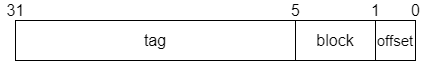
\includegraphics[width=0.4\textwidth]{fig-cache-addr.png}
        \caption{高速缓存地址映射策略}
        \label{fig:cache-addr}
    \end{figure}
    高速缓存模块输入输出信号如表\ref{tab:cache-input-output-sig}所示。
    \begin{table}[htbp]
        \centering
        \begin{tabular}{|c|c|c|}
        \hline
        输入信号 & 长度 & 说明 \\ \hline
        address & 32 & 内存地址 \\
        writeData & 32 & 写入数据 \\
        memWrite & 1 & 内存写使能信号 \\
        memRead & 1 & 内存读使能信号 \\
        clk & 1 & 时钟信号 \\
        \hline
        \hline
        输出信号 & 长度 & 说明 \\ 
        \hline
        readData & 32 & 内存读取结果\\
        \hline
        \end{tabular}
        \caption{高速缓存模块输入、输出信号}
        \label{tab:cache-input-output-sig}
        \end{table}\par
    本实验中高速缓存模块的输入输出与实验5中内存模块输入输出完全一致,这样的设计出于兼容性考虑,对于外部电路而言,使用高速缓存与直接使用内存模块在接口上没有差异,便于我们将本高速缓存模块安装在其他系统上。

\subsubsection{内存单元模块}
    内存(Memory)是计算机的重要部件之一,也称内存储器和主存储器,它用于暂时存放CPU中的运算数据,与硬盘等外部存储器交换的数据。 它是外存与CPU进行沟通的桥梁,计算机中所有程序的运行都在内存中进行,内存性能的强弱影响计算机整体发挥的水平。\par
    在本实验中,内存单元模块按字进行寻址,同时,我们不考虑页表、虚拟地址与物理地址的转化,只考虑直接操作物理地址的情况。实验中我们的内存大小设定为1024个字,但是为了契合一般的处理器设计,我们的内存模块依然能接受32位地址输入,但是仅当内存地址小于1024时,内存操作才是有效的。\par
    与实验5不同,本实验中我们加入了高速缓存,为了与高速缓存模块对接,本实验中的内存单元模块将会一次性返回4个字的内容。\par
    内存模块输入输出信号如表\ref{tab:mem-input-output-sig}所示。
    \begin{table}[htbp]
        \centering
        \begin{tabular}{|c|c|c|}
        \hline
        输入信号 & 长度 & 说明 \\ \hline
        address & 32 & 内存地址 \\
        writeData & 32 & 写入数据 \\
        memWrite & 1 & 内存写使能信号 \\
        memRead & 1 & 内存读使能信号 \\
        clk & 1 & 时钟信号 \\
        \hline
        \hline
        输出信号 & 长度 & 说明 \\ 
        \hline
        readData & 128 & 内存读取结果\\
        \hline
        \end{tabular}
        \caption{内存模块输入、输出信号}
        \label{tab:mem-input-output-sig}
        \end{table}\par
    与寄存器模块即时响应读取操作不同,内存模块仅在memRead处于高电平时才会进行读取操作。写入操作与寄存器模块相似,内存模块会在时钟下降沿且memWrite信号为高电平时,将writeData值写入address地址。

\subsubsection{符号扩展模块}
    符号扩展模块可以根据主控制器模块(Ctr)的信号,以带符号扩展或无符号扩展对来自指令的16位数进行扩展,扩展结果为一个32位的数。\par
    符号扩展模块的输入输出信号如表\ref{tab:signext-input-output-sig}所示。
    \begin{table}[htbp]
        \centering
        \begin{tabular}{|c|c|c|}
        \hline
        输入信号 & 长度 & 说明 \\ 
        \hline
        inst & 16 & 指令中的立即数 \\
        signExt & 1 & 高电平代表进行带括号扩展,否则无符号扩展 \\
        \hline
        \hline
        输出信号 & 长度 & 说明 \\ 
        \hline
        data & 32 & 扩展结果\\
        \hline
        \end{tabular}
        \caption{符号扩展模块输入、输出信号}
        \label{tab:signext-input-output-sig}
        \end{table}
    
\subsubsection{数据选择器模块(Mux/RegMux)}
    数据选择器模块接受两个输入信号和一个选择信号,产生一个输出信号。本实验中,我们使用了两种数据选择器,包括Mux和RegMux。Mux的输入与输出信号均为32位,用于对进行数据进行选择。RegMux的输入和输出信号为5位,用于寄存器选取信号的选择。\par
    数据选择器的电路模型如图\ref{fig:mux}所示。\par
    \begin{figure}[H]
        \centering
        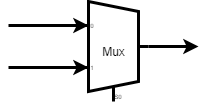
\includegraphics[width=0.2\textwidth]{fig-mux.png}
        \caption{数据选择器的电路模型}
        \label{fig:mux}
    \end{figure}

\subsubsection{指令内存模块(InstMem)}
    本实验中处理器采用哈佛架构,指令内存与数据内存分离。指令内存模块(InstMem)接受一个32位地址输入,输出一条32位指令。

\subsection{流水线阶段原理分析}
\subsubsection{取指令阶段(IF)}
    取指令阶段主要包括PC寄存器与指令内存模块,此阶段指令内存模块根据PC寄存器的值取出指令。
\subsubsection{译码阶段(ID)}
    译码阶段主要包括主控制器模块(Ctr)、寄存器模块(Register)、符号扩展模块。主控制器产生控制信号,寄存器模块读取寄存器数据,符号扩展模块将立即数扩展为32位。同时,在此阶段目标寄存器选择器还会在rt与rd中选择出写入寄存器,此阶段仅选择出写入寄存器后并不会执行写操作,选择结果会一直保存到WB阶段进行实际写入。提前完成写入寄存器选择工作,既便于之后的数据保存、传输,也方便进行数据冒险判断与前向通路实现。\par
    对于无条件跳转指令j、jal、jr,其对应的所有操作都会在本阶段完成,以此来提高流水线的执行效率。
\subsubsection{执行阶段(EX)}
    执行阶段主要包括ALU控制器(ALUCtr)、ALU以及一系列用于选择ALU输入数据的选择器。本阶段中ALU会根据ALU控制器的控制信号与输入数据计算出结果,对于beq、bne指令,本阶段也会决定是否跳转。\par
    对于lui指令,lui选择器会选取指令中立即数部分作为本阶段的执行结果的高16位,ALU的计算结果在此指令下会被丢弃。
\subsubsection{访存阶段(MA)}
    访存阶段主要包括高速缓存模块,高速缓存模块与内存模块相连,用以加速内存操作。对于需要进行访存的指令,将在本阶段完成访存操作。本阶段还有一个数据选择器,该选择器根据MEM\_TO\_REG控制信号,在访存结果与执行阶段结果中选择一个数据作为访存阶段的结果。
\subsubsection{写回阶段(WB)}
    写回阶段主要包括寄存器模块,对于需要寄存器写入的指令,本阶段将完成寄存器写操作。其中,写入寄存器的编号在ID阶段已经确定,写入的数据为MA阶段的结果。

\subsection{顶层模块(top)原理分析}\label{sec:design-top}
\subsubsection{段寄存器}
    在流水线的两个阶段之间,需要通过段寄存器临时保存上一阶段的执行结果和控制信号。
    \begin{itemize}
        \item IF-ID 段寄存器:主要包含当前指令内容及PC
        \item ID-EX 段寄存器:主要包含控制信号、符号扩展的结果,rs、rt对应寄存器的编号,目标写入寄存器的编号,funct、shamt的值、当前指令PC
        \item EX-MA 段寄存器:主要包含控制信号、ALU的运算结果、rt寄存器的编号以及目标写入寄存器的编号
        \item MA-WB 段寄存器:主要包含regWrite控制信号、最终写入寄存器的数据以及目标写入寄存器的编号
    \end{itemize}
    控制信号在段之间的传递关系如图\ref{fig:design-top-ctr-sig}所示。
    \begin{figure}[H]
        \centering
        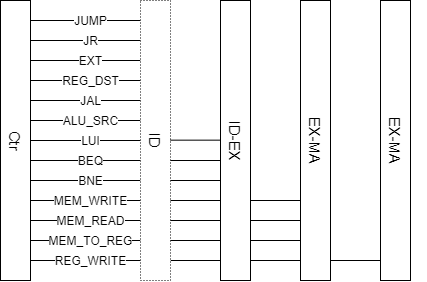
\includegraphics[width=0.45\textwidth]{fig-design-top-ctr-sig}
        \caption{控制信号的传递关系}
        \label{fig:design-top-ctr-sig}
    \end{figure}
\subsubsection{数据前向传递原理分析}
    在流水线中,当前指令在EX阶段所需要的数据可能来自先前指令的写回结果,但是被依赖的指令可能才刚开始MA阶段或WB阶段。尽管当前指令可以等待依赖指令完全执行结束再从寄存器中获得需要的数据,但是这样的策略会导致大量流水线停滞,降低处理器效率。通过添加前向数据通路,从EX-MA段寄存器、MA-WB段寄存器获得需要的数据,可以不需要等待先前指令完成WB阶段,由此提高效率。
\subsubsection{停顿机制原理分析}
    对于“读内存-使用”型数据冒险,前向传递无法避免停顿,这是由于lw指令需要在MA阶段完成后才能得到需要的数据,而下一条指令必须在EX阶段开始前获得需要的数据。因此,后一条指令必须在EX阶段开始前等待一个周期,待lw指令完成MA阶段后,使用前向数据通路将访存结果送回EX阶段。\par
    在每条指令的ID阶段,我们均会检测该指令是否和前一条指令形成“读内存-使用”型数据冒险,如果存在这样的冒险,则发出STALL信号,使得IF、ID阶段停顿一个周期。
\subsubsection{分支预测原理分析}\label{sec:design-branch-predict}
    对于跳转指令,我们通过预测不转移(predict-not-taken)来解决条件转移带来的控制竞争,即对于所有的指令均预测不会跳转,当预测错误时,则生成NOP信号请求清空IF、ID阶段。这种策略的正确性需要分情况说明:
    \begin{itemize}
        \item \textbf{无条件跳转指令:}这类指令会在ID阶段完成跳转,产生的NOP信号会清空ID-EX段寄存器,即跳转指令本身会在ID阶段结束后被清除,但由于跳转指令在ID阶段就已经完成了所有工作,因此并不会导致执行错误。
        \item \textbf{条件跳转指令:}这类指令会在EX阶段完成跳转,当跳转发生时,IF、ID阶段的指令由于预测错误,理应被清除,因此在此情况下,我们的清除策略也是正确的。
    \end{itemize}
    在此,有以下两点需要特别说明:
    \begin{itemize}
        \item 当IF-ID段寄存器接收到NOP信号时,并不一定会清空段寄存器,此处我们额外加入了当前指令地址和跳转目标PC的比较,当两者相同时,指令会正常执行。这样的设计可以为短跳转(例如仅跳过一行指令的条件跳转)减少一个停顿周期。
        \item 在跳转目标PC的选择电路中,我们将条件跳转(beq、bne)的选择器安排在无条件跳转之后。这样的设计,当条件跳转语句后紧跟非条件跳转时,保证了跳转目标PC的正确性。
    \end{itemize}
\subsubsection{jal指令实现原理分析}
    如先前所说,无条件跳转语句会在ID阶段完成所有工作,但是jal指令由于需要进行寄存器写入,可能会与处于WB阶段的指令产生结构冒险。为解决这个问题,处理jal指令时,将当前处于EX、MA、WB阶段的指令全部停顿一个周期,为jal指令让出寄存器写入端口。由于jal使用的31号寄存器不是通用寄存器,其余指令不会对此寄存器进行写入,改变寄存器写入顺序不会导致数据错误。

\section{功能实现}\label{sec-imp}

\subsection{功能模块的实现}
\subsubsection{主控制器模块的实现}
本实验中,主控制器模块(Ctr)的输出结果由指令中opCode段决定。通过case语句,我们可以将指令与opCode对应,并根据每个指令的操作需求输出控制信号。\par
主控制器模块的完整实现见Ctr.v,相比实验5中实现代码,本实验中增加了部分跳转指令与lui指令的控制信号,同时将jrSign信号的产生集成到主控制器模块中。部分核心代码如下:
\begin{lstlisting}[language=verilog]
always @(opCode or funct)
begin
    case(opCode)
    6'b000000: //R type
    begin
        RegDst = 1;
        ALUSrc = 0;
        MemToReg = 0;
        MemRead = 0;
        MemWrite = 0;
        BeqSign = 0;
        BneSign = 0;
        ExtSign = 0;
        LuiSign = 0;
        JalSign = 0;
        ALUOp = 3'b101;
        JumpSign = 0;
        if (funct == 6'b001000) begin
            RegWrite = 0;
            JrSign = 1;
        end else begin
            RegWrite = 1;
            JrSign = 0;
        end
    end
    6'b100011: //lw
    begin
        RegDst = 0;
        ALUSrc = 1;
        MemToReg = 1;
        RegWrite = 1;
        MemRead = 1;
        MemWrite = 0;
        BeqSign = 0;
        BneSign = 0;
        ExtSign = 1;
        LuiSign = 0;
        JalSign = 0;
        ALUOp = 3'b000;
        JumpSign = 0;
        JrSign = 0;
    end
    //后续代码类似,此处省略
    endcase
end
\end{lstlisting}
受限于篇幅,此处只展示R型指令与lw指令对应的实现。\par
代码中RegDst、ALUSrc、MemToReg等为控制信号寄存器,与对应输出信号线相连。

\subsubsection{ALU控制器模块的实现}
ALU控制器模块(ALUCtr)的输出由aluOp与funct共同决定,其行为与主控制器模块(Ctr)相似。不同的是,aluOp与funct有部分位在部分指令中属于无关的位,因此我们使用casex替代case。casex中,可以用x表示我们不关心的位。\par
ALU控制器模块的完整实现见ALUCtr.v,相比实验5中实现,本实验中ALU控制器模块不再产生jrSign信号。核心代码如下:
\begin{lstlisting}[language=verilog]
always @ (aluOp or funct)
begin
    ShamtSign = 0;
    casex({aluOp,funct})
        9'b000xxxxxx:  // lw,sw,add,addiu
            ALUCtrOut = 4'b0010;    //add
        9'b001xxxxxx:  // beq,bne
            ALUCtrOut = 4'b0110;    //sub
        9'b010xxxxxx:   //stli
            ALUCtrOut = 4'b0111;
        9'b110xxxxxx:   //stliu
            ALUCtrOut = 4'b1000;
        9'b011xxxxxx:  // andi
            ALUCtrOut = 4'b0000;
        9'b100xxxxxx:  // ori
            ALUCtrOut = 4'b0001;
        9'b111xxxxxx:  // xori
            ALUCtrOut = 4'b1011;
        
        //R type
        9'b101001000:  // jr
            ALUCtrOut = 4'b0101;
        9'b101000000:  // sll
        begin
            ALUCtrOut = 4'b0011;
            ShamtSign = 1;
        end
        9'b101000010:  // srl
        begin
            ALUCtrOut = 4'b0100;
            ShamtSign = 1;
        end
        9'b101000011:  // sra
        begin
            ALUCtrOut = 4'b1110;
            ShamtSign = 1;
        end
        9'b101000100:  // sllv
            ALUCtrOut = 4'b0011;
        9'b101000110:  // srlv
            ALUCtrOut = 4'b0100;
        9'b101000111:  // srav
            ALUCtrOut = 4'b1110;
        9'b101100000:  // add
            ALUCtrOut = 4'b0010;
        9'b101100001:  // addu
            ALUCtrOut = 4'b0010;
        9'b101100010:  // sub
            ALUCtrOut = 4'b0110;
        9'b101100011:  // subu
            ALUCtrOut = 4'b0110;
        9'b101100100:  // and
            ALUCtrOut = 4'b0000;
        9'b101100101:  // or
            ALUCtrOut = 4'b0001;
        9'b101100110:  // xor
            ALUCtrOut = 4'b1011;
        9'b101100111:  // nor
            ALUCtrOut = 4'b1100;
        9'b101101010:  // slt
            ALUCtrOut = 4'b0111;
        9'b101101011:  // sltu
            ALUCtrOut = 4'b1000;
    endcase
end
\end{lstlisting}

\subsubsection{ALU模块的实现}
ALU模块根据aluCtr信号完成指定的功能,可以使用case语句选择操作,利用verilog自带的运算符完成运算。\par
ALU模块的完整实现见ALU.v,本实验ALU模块实现与实验5完全一致,核心代码如下:
\begin{lstlisting}[language=verilog]
always @ (input1 or input2 or aluCtr)
begin
    case(aluCtr)
    4'b0000:    //AND
        ALURes = input1 & input2;
    4'b0001:    //OR
        ALURes = input1 | input2;
    4'b0010:    //ADD
        ALURes = input1 + input2;
    4'b0011:    //Left-shift
        ALURes = input2 << input1;
    4'b0100:    //Right-shift
        ALURes = input2 >> input1;
    4'b0101:
        ALURes = input1;
    4'b0110:    //SUB
        ALURes = input1 - input2;
    4'b0111:    //SLT
        ALURes = ($signed(input1) < $signed(input2));
    4'b1000:    //SLTU
        ALURes = (input1 < input2);
    4'b1011:    //xor
        ALURes = input1 ^ input2;
    4'b1100:    //nor
        ALURes = ~(input1 | input2);
    4'b1110:    //Right-shift-arithmetic
        ALURes = ($signed(input2) >> input1);
    endcase
    if(ALURes==0)
        Zero = 1;
    else
        Zero = 0;
end
\end{lstlisting}\par
SLT运算功能的实现中,由于Verilog会默认以无符号数解释wire类型,需要通过\$signed关键词将输入解释为带符号数后再进行比较。\par
在ALU模块的结尾,我们判断运算结果是否为0,并以此设置Zero寄存器,最终作为zero信号输出。

\subsubsection{寄存器模块的实现}
寄存器会一直进行读操作,而由regWrite控制写操作。为实现信号同步,保证信号的完整性,写操作仅在时钟下降沿进行。由于读操作即时进行,寄存器内容被修改后,对应寄存器的读取结果也会同时更新。\par
相比与实验4中的实现,本实验中寄存器模块可以响应reset信号,当reset为高电平时,所有寄存器清零。\par
寄存器模块的完整实现见Registers.v,核心部分代码如下:
\begin{lstlisting}[language=verilog]
reg [31:0] RegFile[31:0];
integer i;

initial begin
    RegFile[0] = 0;
end

assign readData1 = RegFile[readReg1];
assign readData2 = RegFile[readReg2];

always @ (negedge clk or reset)
begin
    if(reset)
    begin
        for(i=0;i<32;i=i+1)
            RegFile[i] = 0;
    end
    else begin
        if(regWrite)
            RegFile[writeReg] = writeData; 
    end
end
\end{lstlisting}

\subsubsection{内存单元模块的实现}
内存模块由memRead控制是否进行读取操作,当memRead或address信号发生变化或时钟处于下降沿时,内存模块会根据address指定的内存地址内容更新数据读取数据,并将其作为结果输出。本模块中,内存单元模块与高速缓存模块协同工作,内存模块会一次性返回连续4个字的数据。\par
写操作由memWrite信号控制。与寄存器模块相似,为实现信号同步,保证信号的完整性,写操作仅在时钟下降沿进行。\par
内存模块的完整实现见dataMemory.v,核心部分代码如下:
\begin{lstlisting}[language=verilog]
reg [31:0] memFile [0:1023];
reg [127:0] ReadData;
always @(memRead or address or memWrite) 
begin
    if(memRead)
    begin
        if(address<1023)
            ReadData = {memFile[address],memFile[address+1],memFile[address+2],memFile[address+3]};
        else
            ReadData = 0;
    end
end

always @(negedge clk)
begin
    if(memWrite)
        if(address<1023)
            memFile[address] = writeData;
end

assign readData = ReadData;
\end{lstlisting}

\subsubsection{高速缓存模块的实现}
对于外部系统而言,高速缓存模块的接口与普通内存模块没有差异。进行读操作时,高速缓存模块会首先检查缓存是否有效,若缓存失效则从内存读取数据并保存至缓存。进行写操作时,直接写入内存模块,同时将缓存中对应块标记为无效。\par
当缓存失效而从内存读取数据时,需要添加延时以等待内存模块完成读取操作,待内存模块读取完成且缓存块更新之后再输出读取结果。\par
高速缓存模块的完整实现见Cache.v,核心部分代码如下:
\begin{lstlisting}[language=verilog]
reg[31:0] cacheFile[0:63];
reg validBit[0:15];
reg[25:0] tag[0:15];

reg[31:0] ReadData;

wire[127:0] dataFromMemFile;

wire[3:0] cacheAddr = address[5:2];
wire[31:0] MemFileAddress = {address[31:2],2'b00};
integer i;
dataMemory mem(
    .clk(clk),
    .address(MemFileAddress),
    .writeData(writeData),
    .memWrite(memWrite),
    .memRead(memRead),
    .readData(dataFromMemFile)
);

initial 
begin
    for(i=0;i<64;i=i+1)
        validBit[i] = 1'b0;
        tag[i] = 16'b0;
end

always @(memRead or address or memWrite) 
begin
    if(memRead)
    begin
        if(validBit[cacheAddr] & tag[cacheAddr] == address[31:6])
            ReadData = cacheFile[address[5:0]];
        else begin
            tag[cacheAddr] = address[31:6];
            validBit[cacheAddr] = 1'b1;
            #5
            cacheFile[{cacheAddr,2'b11}] = dataFromMemFile[31:0];
            cacheFile[{cacheAddr,2'b10}] = dataFromMemFile[63:32];
            cacheFile[{cacheAddr,2'b01}] = dataFromMemFile[95:64];
            cacheFile[{cacheAddr,2'b00}] = dataFromMemFile[127:96];
            ReadData = cacheFile[address[5:0]];
        end
    end
end

always @(negedge clk)
begin
    if(memWrite)
        validBit[cacheAddr] = 1'b0;
end

assign readData = ReadData;
\end{lstlisting}\par

\subsubsection{符号扩展模块的实现}
    带符号扩展可以通过在高16位填入立即数第15位实现,无符号扩展可以通过在高16位填入0实现。为了在两种工作模式下切换,可以通过一个三目运算符根据signExt信号在两种扩展结果中进行选择。\par
    符号扩展模块的完整实现见signext.v,核心部分代码如下:
\begin{lstlisting}[language=verilog]
assign data = signExt?{{16{inst[15]}},inst[15:0]}:{{16{0}},inst[15:0]};
\end{lstlisting}

\subsubsection{数据选择器模块的实现}
    使用Verilog自带的三目运算符即可实现数据选择器的功能。Mux与RegMux的差异仅在于输入输出数据长度不同。\par
    数据选择器模块的完整实现见Mux.v与RegMux.v,核心代码如下:
\begin{lstlisting}[language=verilog]
assign out = select?input1:input0;
\end{lstlisting}

\subsubsection{指令内存模块的实现}
    指令内存模块只需要根据PC地址输出对应的指令,实现相对简单。\par
    指令内存模块的完整实现见InstMem.v,核心代码如下:
\begin{lstlisting}[language=verilog]
reg [31:0] instFile[0:1023];
assign inst = instFile[address/4];
\end{lstlisting}

\subsection{顶层模块的实现}

\subsubsection{段寄存器实现}
\begin{lstlisting}[language=verilog]
//IF to ID
reg [31:0] IF2ID_INST;
reg [31:0] IF2ID_PC;
//ID to EX
reg [2:0] ID2EX_ALUOP;
reg [7:0] ID2EX_CTR_SIGNALS;
reg [31:0] ID2EX_EXT_RES;
reg [4:0] ID2EX_INST_RS;
reg [4:0] ID2EX_INST_RT;
reg [31:0] ID2EX_REG_READ_DATA1;
reg [31:0] ID2EX_REG_READ_DATA2;
reg [5:0] ID2EX_INST_FUNCT;
reg [4:0] ID2EX_INST_SHAMT;
reg [4:0] ID2EX_REG_DEST;
reg [31:0] ID2EX_PC;
//EX to MA
reg [3:0] EX2MA_CTR_SIGNALS;
reg [31:0] EX2MA_ALU_RES;
reg [31:0] EX2MA_REG_READ_DATA_2;
reg [4:0] EX2MA_REG_DEST;
//MA to WB
reg MA2WB_CTR_SIGNALS;
reg [31:0] MA2WB_FINAL_DATA;
reg [4:0] MA2WB_REG_DEST;
\end{lstlisting}

\subsubsection{功能模块连接}
每个阶段中的功能模块从段寄存器中获得输入信号,产生输出信号,输出信号将在下一个时钟上升沿写入下一阶段的段寄存器中。\par
以主控制器模块的连接为例,其实现如下:
\begin{lstlisting}[language=verilog]
wire [12:0] ID_CTR_SIGNALS;
wire [2:0] ID_CTR_SIGNAL_ALUOP;
wire ID_JUMP_SIG;
wire ID_JR_SIG;
wire ID_EXT_SIG;
wire ID_REG_DST_SIG;
wire ID_JAL_SIG;
wire ID_ALU_SRC_SIG;
wire ID_LUI_SIG;
wire ID_BEQ_SIG;
wire ID_BNE_SIG;
wire ID_MEM_WRITE_SIG;
wire ID_MEM_READ_SIG;
wire ID_MEM_TO_REG_SIG;
wire ID_REG_WRITE_SIG;
wire ID_ALU_OP;
Ctr main_ctr(
    .opCode(IF2ID_INST[31:26]),
    .funct(IF2ID_INST[5:0]),
    .jumpSign(ID_JUMP_SIG),
    .jrSign(ID_JR_SIG),
    .extSign(ID_EXT_SIG),
    .regDst(ID_REG_DST_SIG),
    .jalSign(ID_JAL_SIG),
    .aluSrc(ID_ALU_SRC_SIG),
    .luiSign(ID_LUI_SIG),
    .beqSign(ID_BEQ_SIG),
    .bneSign(ID_BNE_SIG),
    .memWrite(ID_MEM_WRITE_SIG),
    .memRead(ID_MEM_READ_SIG),
    .memToReg(ID_MEM_TO_REG_SIG),
    .regWrite(ID_REG_WRITE_SIG),
    .aluOp(ID_CTR_SIGNAL_ALUOP)
);
//将信号合并为总线,便于段寄存器读写
assign ID_CTR_SIGNALS[12] = ID_JUMP_SIG;
assign ID_CTR_SIGNALS[11] = ID_JR_SIG;
assign ID_CTR_SIGNALS[10] = ID_EXT_SIG;
assign ID_CTR_SIGNALS[9] = ID_REG_DST_SIG;
assign ID_CTR_SIGNALS[8] = ID_JAL_SIG;
assign ID_CTR_SIGNALS[7] = ID_ALU_SRC_SIG;
assign ID_CTR_SIGNALS[6] = ID_LUI_SIG;
assign ID_CTR_SIGNALS[5] = ID_BEQ_SIG;
assign ID_CTR_SIGNALS[4] = ID_BNE_SIG;
assign ID_CTR_SIGNALS[3] = ID_MEM_WRITE_SIG;
assign ID_CTR_SIGNALS[2] = ID_MEM_READ_SIG;
assign ID_CTR_SIGNALS[1] = ID_MEM_TO_REG_SIG;
assign ID_CTR_SIGNALS[0] = ID_REG_WRITE_SIG;
\end{lstlisting}

\subsubsection{前向通路实现}
当前指令处于EX阶段时,运算输入可能来自先前指令的写回结果,为提高流水线性能,我们引入前向数据通路。进行数据前向传递需要满足以下条件:
\begin{enumerate}
    \item 先前指令需要进行寄存器写入操作。
    \item 先前指令写入的目标寄存器与当前指令的读取寄存器相同。
\end{enumerate}\par
前向数据通路的实现如下:
\begin{lstlisting}[language=verilog]
wire[31:0] EX_FORWARDING_A_TEMP;
wire[31:0] EX_FORWARDING_B_TEMP;
Mux forward_A_mux1(
    .select(WB_REG_WRITE & (MA2WB_REG_DEST == ID2EX_INST_RS)),
    .input0(ID2EX_REG_READ_DATA1),
    .input1(MA2WB_FINAL_DATA),
    .out(EX_FORWARDING_A_TEMP)
);
Mux forward_A_mux2(
    .select(MA_REG_WRITE & (EX2MA_REG_DEST == ID2EX_INST_RS)),
    .input0(EX_FORWARDING_A_TEMP),
    .input1(EX2MA_ALU_RES),
    .out(FORWARDING_RES_A)
);
Mux forward_B_mux1(
    .select(WB_REG_WRITE & (MA2WB_REG_DEST == ID2EX_INST_RT)),
    .input0(ID2EX_REG_READ_DATA2),
    .input1(MA2WB_FINAL_DATA),
    .out(EX_FORWARDING_B_TEMP)
);
Mux forward_B_mux2(
    .select(MA_REG_WRITE & (EX2MA_REG_DEST == ID2EX_INST_RT)),
    .input0(EX_FORWARDING_B_TEMP),
    .input1(EX2MA_ALU_RES),
    .out(FORWARDING_RES_B)
);
\end{lstlisting}\par
代码中forward\_A、forward\_B为两组前项通路,分别用于将数据传输ALU的两个输入端口,每组通路包括两个选择器,分别从EX-MA段寄存器与MA-WB段寄存器获取数据。

\subsubsection{跳转目标PC选择的实现}
我们使用4个数据选择器选择下一个PC地址,负责条件跳转的选择器在无条件跳转的选择器之后,其原因已在\ref{sec:design-branch-predict}节中说明。\par
PC地址选择的实现代码如下:
\begin{lstlisting}[language=verilog]
// ID stage
wire[31:0] PC_AFTER_JUMP_MUX;
Mux jump_mux(
    .select(ID_JUMP_SIG), 
    .input1(((IF2ID_PC + 4) & 32'hf0000000) + (IF2ID_INST [25 : 0] << 2)),
    .input0(IF_PC + 4),
    .out(PC_AFTER_JUMP_MUX)
);

wire[31:0] PC_AFTER_JR_MUX;
Mux jr_mux(
    .select(ID_JR_SIG),   
    .input0(PC_AFTER_JUMP_MUX),
    .input1(ID_REG_READ_DATA1),
    .out(PC_AFTER_JR_MUX)
);

// EX stage
wire EX_BEQ_BRANCH = EX_BEQ_SIG & EX_ALU_ZERO;
wire[31:0] PC_AFTER_BEQ_MUX;
Mux beq_mux(
    .select(EX_BEQ_BRANCH),
    .input1(BRANCH_DEST),
    .input0(PC_AFTER_JR_MUX),
    .out(PC_AFTER_BEQ_MUX)
);

wire EX_BNE_BRANCH = EX_BNE_SIG & (~ EX_ALU_ZERO);
wire[31:0] PC_AFTER_BNE_MUX;
Mux bne_mux(
    .select(EX_BNE_BRANCH),
    .input1(BRANCH_DEST),
    .input0(PC_AFTER_BEQ_MUX),
    .out(PC_AFTER_BNE_MUX)
);
wire[31:0] NEXT_PC = PC_AFTER_BNE_MUX;
wire BRANCH = EX_BEQ_BRANCH | EX_BNE_BRANCH;
\end{lstlisting}

\subsubsection{流水线时序实现}
本部分是流水线处理器实现的核心,段寄存器写入、分支预测、停顿等功能均在本部分实现。\par
各个段寄存器的清空、停顿条件如下:
\begin{itemize}
    \item \textbf{IF-ID段寄存器:}如果NOP信号有效且当前指令地址与目标跳转PC不一致,说明分支预测失败,则清空段寄存器。
    \item \textbf{ID-EX段寄存器:}ID\_JAL\_SIG信号有效时说明当前指令为jal,ID-EX段寄存器维持原样,ID阶段结果不写入段寄存器。STALL信号有效时表明需要停顿,清空ID-EX段寄存器,避免EX阶段执行错误指令。NOP指令有效时说明分支预测错误,清空ID-EX段寄存器。
    \item \textbf{EX-MA段寄存器:}ID\_JAL\_SIG信号有效时说明当前指令为jal,ID之后的阶段需要停顿一个周期,EX-MA段寄存器维持原样。
    \item \textbf{MA-WB段寄存器:}ID\_JAL\_SIG信号有效时说明当前指令为jal,ID之后的阶段需要停顿一个周期,MA-WB段寄存器维持原样。
\end{itemize}\par
流水线时序实现代码如下:
\begin{lstlisting}[language=verilog]
always @(posedge clk) 
begin
    NOP = BRANCH | ID_JUMP_SIG | ID_JR_SIG;
    STALL = ID2EX_CTR_SIGNALS[2] & //该信号来自于ID_MEM_READ_SIG
                ((ID2EX_INST_RT == ID_REG_RS) | 
                (ID2EX_INST_RT == ID_REG_RT)); //如果读取的两个寄存器与内存读冲突则stall

    if(!STALL)
    begin
        if(NOP)
        begin
            if(IF_PC == NEXT_PC)
            begin
                IF2ID_INST <= IF_INST;
                IF2ID_PC <= IF_PC;
                IF_PC <= IF_PC + 4;
            end
            else begin
                IF2ID_INST <= 0;
                IF2ID_PC <= 0;
                IF_PC <= NEXT_PC;
            end
        end
        else begin
            IF2ID_INST <= IF_INST;
            IF2ID_PC <= IF_PC;
            IF_PC <= NEXT_PC;
        end
    end
    
    // ID - EX
    if (!ID_JAL_SIG)
    begin
        if (STALL|NOP)
        begin
            //STALL:下一个周期不进行EX阶段,等待上条指令MA完成
            //BRANCH:发生跳转,从这里截断命令
            //JUMP的决定在ID阶段,不影响
            ID2EX_PC <= IF2ID_PC;
            ID2EX_ALUOP <= 3'b000;
            ID2EX_CTR_SIGNALS <= 0;
            ID2EX_EXT_RES <= 0;
            ID2EX_INST_RS <= 0;
            ID2EX_INST_RT <= 0;
            ID2EX_REG_READ_DATA1 <= 0;
            ID2EX_REG_READ_DATA2 <= 0;
            ID2EX_INST_FUNCT <= 0;
            ID2EX_INST_SHAMT <= 0;
            ID2EX_REG_DEST <= 0;
        end else 
        begin
            ID2EX_PC <= IF2ID_PC;
            ID2EX_ALUOP <= ID_CTR_SIGNAL_ALUOP;
            ID2EX_CTR_SIGNALS <= ID_CTR_SIGNALS[7:0];
            ID2EX_EXT_RES <= ID_EXT_RES;
            ID2EX_INST_RS <= ID_REG_RS;
            ID2EX_INST_RT <= ID_REG_RT;
            ID2EX_REG_DEST <= ID_REG_DEST;
            ID2EX_REG_READ_DATA1 <= ID_REG_READ_DATA1;
            ID2EX_REG_READ_DATA2 <= ID_REG_READ_DATA2;
            ID2EX_INST_FUNCT <= IF2ID_INST[5:0];
            ID2EX_INST_SHAMT <= IF2ID_INST[10:6];
        end
    end

    // EX - MA
    if (!ID_JAL_SIG)
    begin
        EX2MA_CTR_SIGNALS <= ID2EX_CTR_SIGNALS[3:0];
        EX2MA_ALU_RES <= EX_FINAL_DATA;
        EX2MA_REG_READ_DATA_2 <= FORWARDING_RES_B;
        EX2MA_REG_DEST <= ID2EX_REG_DEST;
    end

    // MA - WB
    if (!ID_JAL_SIG)
    begin
        MA2WB_CTR_SIGNALS <= EX2MA_CTR_SIGNALS[0];
        MA2WB_FINAL_DATA <= MA_FINAL_DATA;
        MA2WB_REG_DEST <= EX2MA_REG_DEST;
    end
end
\end{lstlisting}

\section{结果验证}
编写如表\ref{tab:sim-inst}所示的汇编代码进行测试。\par
% Please add the following required packages to your document preamble:
% \usepackage{multirow}
% \usepackage{longtable}
% Note: It may be necessary to compile the document several times to get a multi-page table to line up properly
\begin{longtable}[c]{|c|c|c|p{1.2cm}<{\centering}|p{1.2cm}<{\centering}|p{1.2cm}<{\centering}|}
\hline
\multirow{2}{*}{地址} & \multirow{2}{*}{指令} & \multirow{2}{*}{汇编指令} & \multicolumn{3}{c|}{预期执行结果} \\ \cline{4-6} 
    &  &  & \$0 & \$1 & \$2 \\ \hline
\endfirsthead
%
\endhead
%
0x00 & 00001000000000000000000000000100 & j & \multicolumn{3}{c|}{跳转至0x10} \\ \hline
0x04 & 00000000000000000000000000000000 & nop & \multicolumn{3}{c|}{不执行} \\ \hline
0x08 & 00000000000000000000000000000000 & nop & \multicolumn{3}{c|}{不执行} \\ \hline
0x0c & 00000000000000000000000000000000 & nop & \multicolumn{3}{c|}{不执行} \\ \hline
0x10 & 00001100000000000000000000000110 & jal & \multicolumn{3}{c|}{跳转至0x18, \$31 = 0x14} \\ \hline
0x14 & 00000000000000000000000000000000 & nop & \multicolumn{3}{c|}{空指令} \\ \hline
0x18 & 00111100000000101111111111111111 & lui \$2,65535 & x & -65536 & x \\ \hline
0x1c & 10001100000000010000000000000010 & lw \$1,2(\$0) & 2 & -65536 & x \\ \hline
0x20 & 10001100000000010000000000000011 & lw \$1,3(\$0) & 3 & -65536 & x \\ \hline
0x24 & 10001100000000100000000000000100 & lw \$2,4(\$0) & 3 & 4 & x \\ \hline
0x28 & 00000000001000100001100000100000 & add \$3,\$1,\$2 & 3 & 4 & 7 \\ \hline
0x2c & 00000000001000100001100000100100 & and \$3,\$1,\$2 & 3 & 4 & 0 \\ \hline
0x30 & 00100000000000110000000000000110 & addi \$3,\$0,6 & 3 & 4 & 6 \\ \hline
0x34 & 00000000001000100010000000100010 & sub \$4,\$1,\$2 & \multicolumn{3}{c|}{\$4 = -1} \\ \hline
0x38 & 00000000000000010000100001000000 & sll \$1,\$1,1 & 6 & 4 & 6 \\ \hline
0x3c & 00000000000000110001100011000000 & sll \$3,\$3,3 & 6 & 4 & 48 \\ \hline
0x40 & 00000000001000110000100000100101 & or \$1,\$3,\$1 & 54 & 4 & 48 \\ \hline
0x44 & 00100100000000100000000000000110 & addiu \$2,\$0,6 & 54 & 6 & 48 \\ \hline
0x48 & 00101000010000010000000000000001 & slti \$1,\$1,1 & 0 & 6 & 48 \\ \hline
0x4c & 00110100010000010000000000000001 & ori \$1,\$2,1 & 7 & 6 & 48 \\ \hline
0x50 & 00000000010000110000100000000100 & sllv \$1,\$3,\$2 & 3072 & 6 & 48 \\ \hline
0x54 & 00000000001000100001100000100001 & addu \$3,\$1,\$2 & 3072 & 6 & 3078 \\ \hline
0x58 & 00000000001000100001100000100010 & sub \$3,\$1,\$2 & 3072 & 6 & 3066 \\ \hline
0x5c & 00000000001000100001100000100011 & subu \$3,\$1,\$2 & 3072 & 6 & 3066 \\ \hline
0x60 & 00000000001000100001100000100101 & or \$3,\$1,\$2 & 3072 & 6 & 3078 \\ \hline
0x64 & 00000000001000100001100000100110 & xor \$3,\$1,\$2 & 3072 & 6 & 3078 \\ \hline
0x68 & 00000000001000100001100000100111 & nor \$3,\$1,\$2 & 3072 & 6 & -3079 \\ \hline
0x6c & 00000000001000100001100000101010 & slt \$3,\$1,\$2 & 3072 & 6 & 0 \\ \hline
0x70 & 00000000000000010000100001000011 & sra \$1,\$1,1 & 1536 & 6 & 0 \\ \hline
0x74 & 10101100000000100000000000000001 & sw \$2,1(\$0) & \multicolumn{3}{c|}{内存地址0x01写入数值6}\\ \hline
0x78 & 00000000010000000000100000101011 & sltu \$1,\$0,\$2 & 0 & 6 & 0 \\ \hline
0x7c & 00000000000000100001000001000010 & srl \$2,\$2,2 & 0 & 3 & 0 \\ \hline
0x80 & 00000000010000100001000000000111 & srav \$2,\$2,\$2 & 0 & 0 & 0 \\ \hline
0x84 & 00111000010000100000000000000010 & xori \$2,\$2,2 & 0 & 2 & 0 \\ \hline
0x88 & 00101100010000010000000000000100 & sltiu \$1,\$2,4 & 1 & 2 & 0 \\ \hline
0x8c & 00010000101000000000000000000001 & beq \$5,\$0,1 & \multicolumn{3}{c|}{跳转至0x94} \\ \hline
0x90 & 00010000101000000000000000000001 & beq \$5,\$0,1 & \multicolumn{3}{c|}{不执行} \\ \hline
0x94 & 00010100101000000000000000000001 & bne \$5,\$0,1 & \multicolumn{3}{c|}{不跳转} \\ \hline
0x98 & 00000011111000000000000000001000 & jr \$31 & \multicolumn{3}{c|}{跳转至0x14} \\ \hline
\caption{仿真使用的指令}
\label{tab:sim-inst}\\
\end{longtable}
数据内存的初始值如表\ref{tab:sim-data}所示。\par
\begin{table}[htbp]
    \centering
    \begin{tabular}{|c|c|}
    \hline
    地址 & 数据 \\ \hline
    0x00 & 0x00000000 \\
    0x01 & 0x00000001 \\
    0x02 & 0x00000002 \\
    0x03 & 0x00000003 \\
    0x04 & 0x00000004 \\
    0x05 & 0x00000005 \\ \hline
    \end{tabular}
    \caption{数据内存初始值}
    \label{tab:sim-data}
    \end{table}
在激励文件中载入指令内存与数据内存数据,此处需要根据数据文件具体目录修改路径。\par
\begin{lstlisting}[language=verilog]
$readmemb("E:/course/arclab/lab06/mem_inst.dat",top.inst_mem.instFile);
$readmemh("E:/course/arclab/lab06/mem_data.dat",top.memory.mem.memFile);
\end{lstlisting}\par
仿真结果如图\ref{fig:sim-res}所示。需要特别说明的是,由于显示缩放问题,部分数字可能没有显示完整。
\begin{figure}[H]
    \centering
    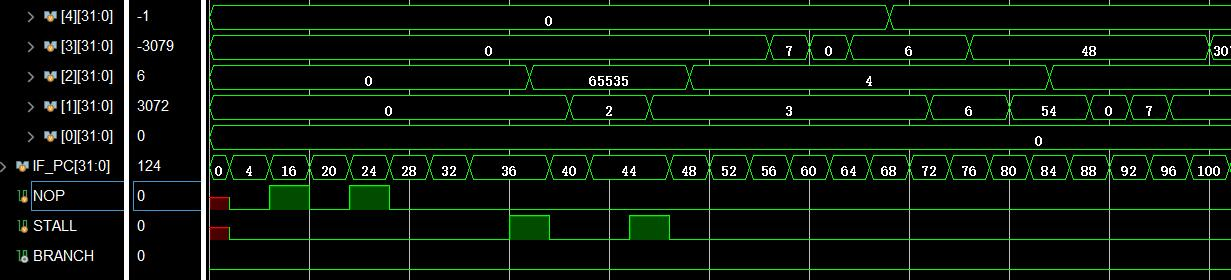
\includegraphics[width=\textwidth]{fig-lab6-sim1.jpg}
    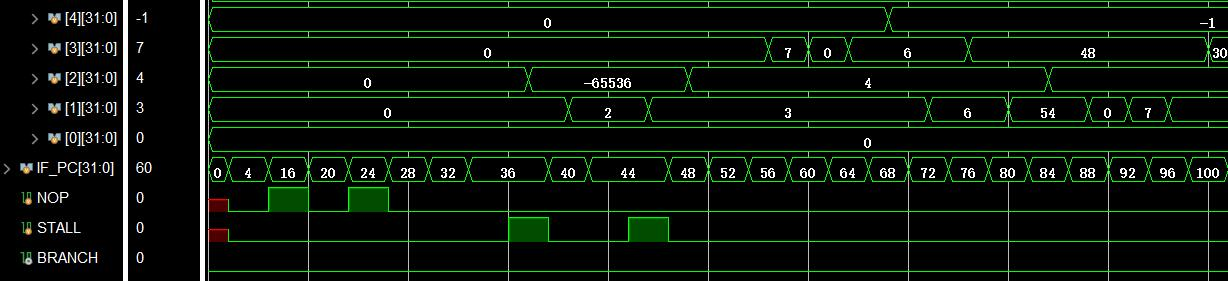
\includegraphics[width=\textwidth]{fig-lab6-sim2.jpg}
    \caption{仿真截图}
    \label{fig:sim-res}
\end{figure}\par
可以看出,我们实现的类MIPS流水线处理器完成了设计的所有功能,执行结果符合预期。

\section{总结与反思}
本实验综合先前5个实验,完成了类MIPS流水线处理器的实现。在实验开始之前,我对流水线的实现毫无头绪,当时的我认为实现流水线处理器是一个毫无可能的任务;实验开始后,在实验指导书的提示下,我将复杂的流水线结构分解,逐一实现每个阶段的线路连接,我发现每个阶段的实现与单周期处理器非常接近,在此之后,只需要将线路整体连接到段寄存器上即可以实现基础的流水线。在完成基础的流水线之后,逐步添加前向通路、停顿、分支预测就显得相对简单。最终,我完成了整个流水线。\par
通过本实验,我加深了对流水器处理器结构的记忆与理解。调试段寄存器时序的过程,让我更加熟悉Verilog的语法以及Vivado软件的仿真调试功能。编写仿真指令的过程,我熟悉了各类MIPS指令的结构、功能与实现原理。完成实验报告的过程,让我对latex的使用更加熟练,也积累了使用Latex编写中文文章的经验。\par
最后,我想向计算机系统结构实验(CS145)的指导老师与助教、计算机系统结构课程(CS359)的授课老师以及实验过程中帮助过我的同学表示由衷的感谢,感谢你们的帮助与陪伴。
\end{document}